\documentclass[]{article}
\usepackage{lmodern}
\usepackage{amssymb,amsmath}
\usepackage{ifxetex,ifluatex}
\usepackage{fixltx2e} % provides \textsubscript
\ifnum 0\ifxetex 1\fi\ifluatex 1\fi=0 % if pdftex
  \usepackage[T1]{fontenc}
  \usepackage[utf8]{inputenc}
\else % if luatex or xelatex
  \ifxetex
    \usepackage{mathspec}
  \else
    \usepackage{fontspec}
  \fi
  \defaultfontfeatures{Ligatures=TeX,Scale=MatchLowercase}
\fi
% use upquote if available, for straight quotes in verbatim environments
\IfFileExists{upquote.sty}{\usepackage{upquote}}{}
% use microtype if available
\IfFileExists{microtype.sty}{%
\usepackage{microtype}
\UseMicrotypeSet[protrusion]{basicmath} % disable protrusion for tt fonts
}{}
\usepackage[margin=1in]{geometry}
\usepackage{hyperref}
\hypersetup{unicode=true,
            pdftitle={Data Analysis},
            pdfborder={0 0 0},
            breaklinks=true}
\urlstyle{same}  % don't use monospace font for urls
\usepackage{graphicx,grffile}
\makeatletter
\def\maxwidth{\ifdim\Gin@nat@width>\linewidth\linewidth\else\Gin@nat@width\fi}
\def\maxheight{\ifdim\Gin@nat@height>\textheight\textheight\else\Gin@nat@height\fi}
\makeatother
% Scale images if necessary, so that they will not overflow the page
% margins by default, and it is still possible to overwrite the defaults
% using explicit options in \includegraphics[width, height, ...]{}
\setkeys{Gin}{width=\maxwidth,height=\maxheight,keepaspectratio}
\IfFileExists{parskip.sty}{%
\usepackage{parskip}
}{% else
\setlength{\parindent}{0pt}
\setlength{\parskip}{6pt plus 2pt minus 1pt}
}
\setlength{\emergencystretch}{3em}  % prevent overfull lines
\providecommand{\tightlist}{%
  \setlength{\itemsep}{0pt}\setlength{\parskip}{0pt}}
\setcounter{secnumdepth}{0}
% Redefines (sub)paragraphs to behave more like sections
\ifx\paragraph\undefined\else
\let\oldparagraph\paragraph
\renewcommand{\paragraph}[1]{\oldparagraph{#1}\mbox{}}
\fi
\ifx\subparagraph\undefined\else
\let\oldsubparagraph\subparagraph
\renewcommand{\subparagraph}[1]{\oldsubparagraph{#1}\mbox{}}
\fi

%%% Use protect on footnotes to avoid problems with footnotes in titles
\let\rmarkdownfootnote\footnote%
\def\footnote{\protect\rmarkdownfootnote}

%%% Change title format to be more compact
\usepackage{titling}

% Create subtitle command for use in maketitle
\newcommand{\subtitle}[1]{
  \posttitle{
    \begin{center}\large#1\end{center}
    }
}

\setlength{\droptitle}{-2em}

  \title{Data Analysis}
    \pretitle{\vspace{\droptitle}\centering\huge}
  \posttitle{\par}
    \author{}
    \preauthor{}\postauthor{}
    \date{}
    \predate{}\postdate{}
  
\usepackage{booktabs}
\usepackage{longtable}
\usepackage{array}
\usepackage{multirow}
\usepackage[table]{xcolor}
\usepackage{wrapfig}
\usepackage{float}
\usepackage{colortbl}
\usepackage{pdflscape}
\usepackage{tabu}
\usepackage{threeparttable}
\usepackage{threeparttablex}
\usepackage[normalem]{ulem}
\usepackage{makecell}

\begin{document}
\maketitle

\hypertarget{description-of-the-problem}{%
\paragraph{\texorpdfstring{\textbf{Description of the
Problem}}{Description of the Problem}}\label{description-of-the-problem}}

We were given 30 State of the Nation (SONA) speeches from 1994 to 2018
to analyse. The specific objectives are to: 1. Infer sentiment and
changes in sentiment over time\\
2. Describe the topics that emerge\\
3. Predict the President from a given sentence of text\\
4. Evaluate out of sample performance of the predictions

\hypertarget{approach}{%
\paragraph{\texorpdfstring{\textbf{Approach}}{Approach}}\label{approach}}

We collaborated using the following GitHub location:
\textbf{\url{https://github.com/samperumal/dsi-assign2}}.

We initially split the work as follows and each of us created a folder
with our names to push our work to for others to view:\\
- Neural Net - Sam and Merve - Bag of Words - Merve - Topic Modelling -
Vanessa - Sentiment Analysis - Audrey

We presented our work to each other and made suggestions for
improvement. Before diving into any prediction, we felt it is important
to do an Exploratory Data Analysis (EDA) to get a sense of the high
level overview of the dataset. This was done by Audrey.

The initial results from the Neural Net gave a 65\% accuracy on the
validation set and we wanted to feed the results of the Topic Modelling
and Sentiment Analysis into the Neural Net to see if it would improve
results so we needed to understand from each other what the output of
these 2 methods was and the input required by the neural net to get the
data into a useable format which took some discussion and a few
iterations.

Given the low accuracy of the neural net (NN), we also tried a
Convolutional Neural Net (CNN). Sam got the initial model working. Merve
made improvements. Vanessa tuned the hyperparamters. \ldots{}need more
here\ldots{}

The cnn did not provide much improvement over the NN so we also tried a
Recurrent Neural Net (RNN) which takes in sequences of data so the order
of the words is also taken into account in the model. \ldots{}need more
here\ldots{}

\hypertarget{data-preparation}{%
\paragraph{Data Preparation}\label{data-preparation}}

Initially we each performed our own import of the data, splitting out
the year and president and tokenisation but we realised there was
duplication of effort here and different naming conventions which made
it difficult to collaborate and use each other's output. In addition,
Sam noticed that some of the data was not being read in because of
special characters and sentences were not being tokenised correctly for
various reasons so he became responsible for performing the data clean
up (preprocessing) and outputting a .RData file that we could all then
use to rerun our work.

The data as provided consisted of 30 text files, with filenames encoding
the president's name, the year of the speech, and whether it was
pre/post an election (which is absent in non-election years). In working
through the files, we discovered that two files were identical which was
corrected in the data source with replacement. Additionally, in reading
the files, we also identified 3 files that had one or more bytes which
caused issues with the standard R file IO routines. Specifically 1 file
had a leading Byte-Order-Mark (BOM) which is unique to windows operating
system files, and 2 other files had invalid unicode characters, which
suggests a text-to-speech processing application was used and
experienced either transmissionor storage errors. In all the cases the
offending characters were simply removed from the input files.

Having fixed basic read issues, we then examined the content of each
file and the simplistic tokenisation achieved by applying
\emph{unnest\_tokens} to the raw lines read in from the files. Several
issues were uncovered, and in each case a \textbf{regular expression}
was created to correct the issue in the raw read lines:

\begin{itemize}
\item
  There are multiple characters which are not handled correctly by the
  default parser, particularly where unicode characters are substituted
  for standard ASCII characters or are erroneously inserted as part of
  the text capture. This range of characters were simply removed from
  the text: \textbf{"``''\%'`\href{}{}--+¬\textgreater{}-}.
\item
  Forward-slashes were converted to a space, to handle both options
  (hot/cold) and numeric ranges (1998/99).
\item
  Bullet-pointed lists are interpreted as a single, exceptionally long
  sentence by default. We chose to split this up into a lead-in sentence
  terminated by a colon, and a list of sentences starting after the
  bullet point character (*).
\item
  Numbers (both with and without thousand separator characters) and
  currency values with leading currency symbols (R/\$) were removed.
\item
  Specific punctuation (ellipsis, colon, semi-colon) was considered
  equivalent to a sentence separator and converted to a full stop:
  \textbf{:;\ldots{}¦\ldots{}}.
\item
  Full stops separated by only whitespace were considered redundany and
  collapsed to a single whitespace character.
\item
  All contiguous whitespace was collapsed to a single whitespace
  character.
\item
  The \emph{unnest\_tokens} function relies on each new sentence
  starting with a capital letter. After the above fixes, it was was
  therefore necessary to capitalise every character after full stop, to
  ensure it is recognised as the start of a new sentence.
\end{itemize}

Having fixed the text to allow correct sentence tokenisation, and
applied the \emph{unnest\_tokens} function, we then determined a unique
ID for each sentence by applying a hash digest function to the sentence
text. This unique ID allowed everyone to work on the same data with
confidence, and also enabled us to detect 72 sentences that appeared
identically in at least 2 speeches. As these duplicates would
potentially bias the analysis and training, all instances of duplicates
were removed from the dataset.

One final note is that each speech starts with a very similar boiler
plate referencing various attendees to the SONA in a single, run-on
sentence. We believe this header does not add significantly to the
content of the speech, and so we excluded all instances across all
speeches.

\begin{figure}
\centering
\includegraphics{DSI_Assignment2_Final_Report_files/figure-latex/unnamed-chunk-1-1.pdf}
\caption{Change in number of sentences per president before and after
filtering.}
\end{figure}

The figure above shows the change in number of sentences per president
after filtering. On the whole there are more sentences per president,
with only a single reduction. Additionally, the highest increases are
associated with the files where read-errors prevented us from previously
reading the entire file. This change is equally evident in the boxplots
below, which show the change in distribution per president of words and
characters per sentence.
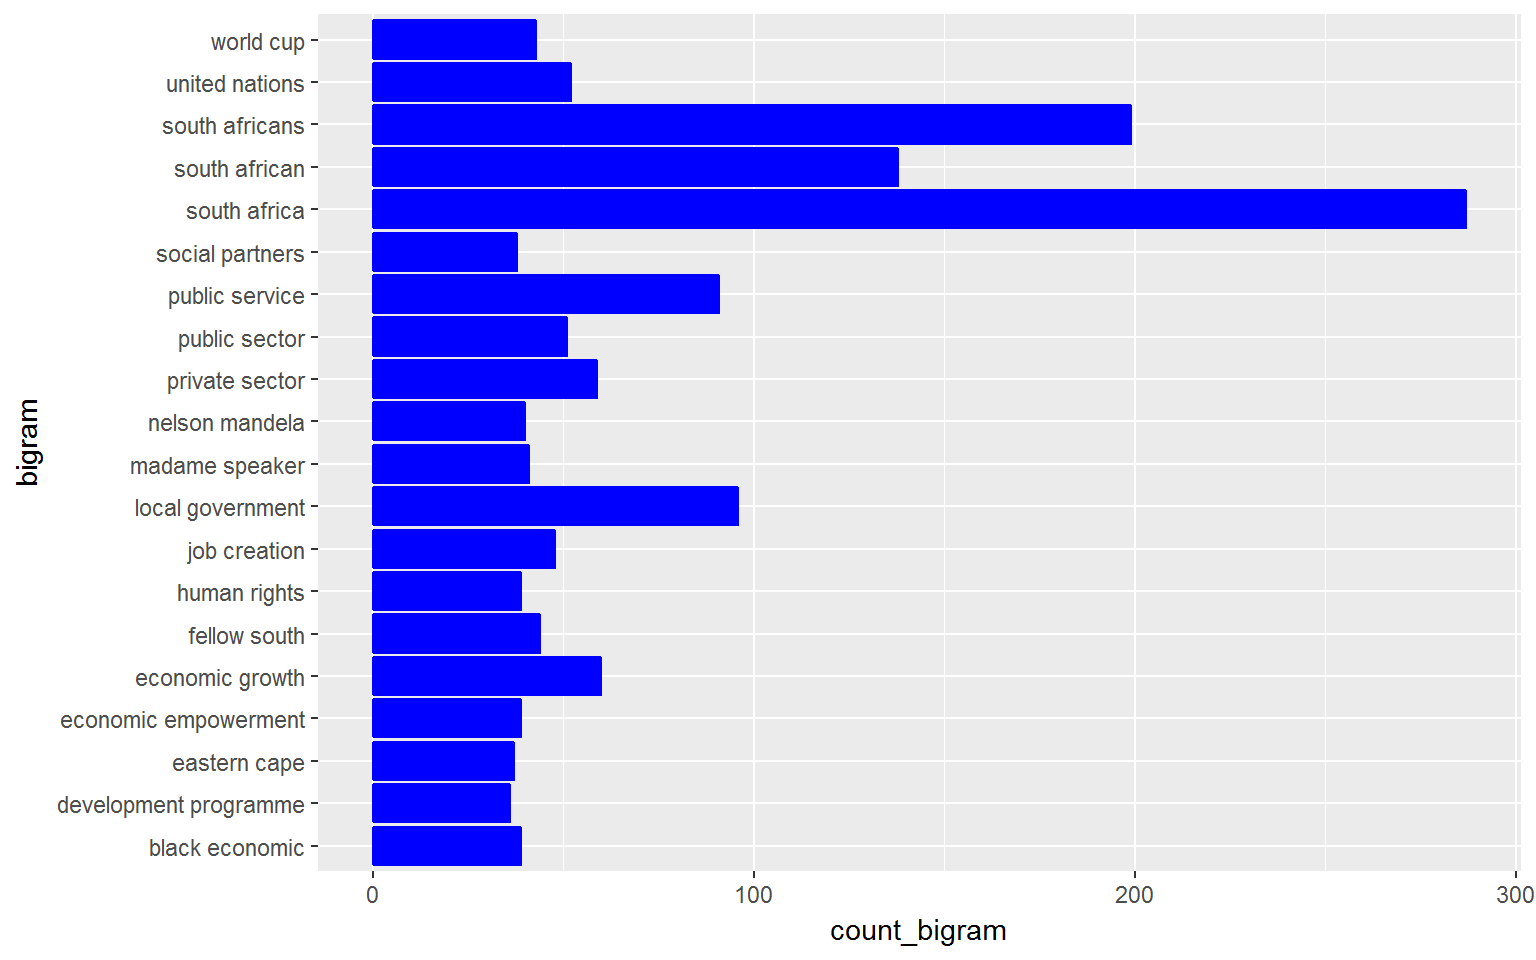
\includegraphics{DSI_Assignment2_Final_Report_files/figure-latex/unnamed-chunk-2-1.pdf}

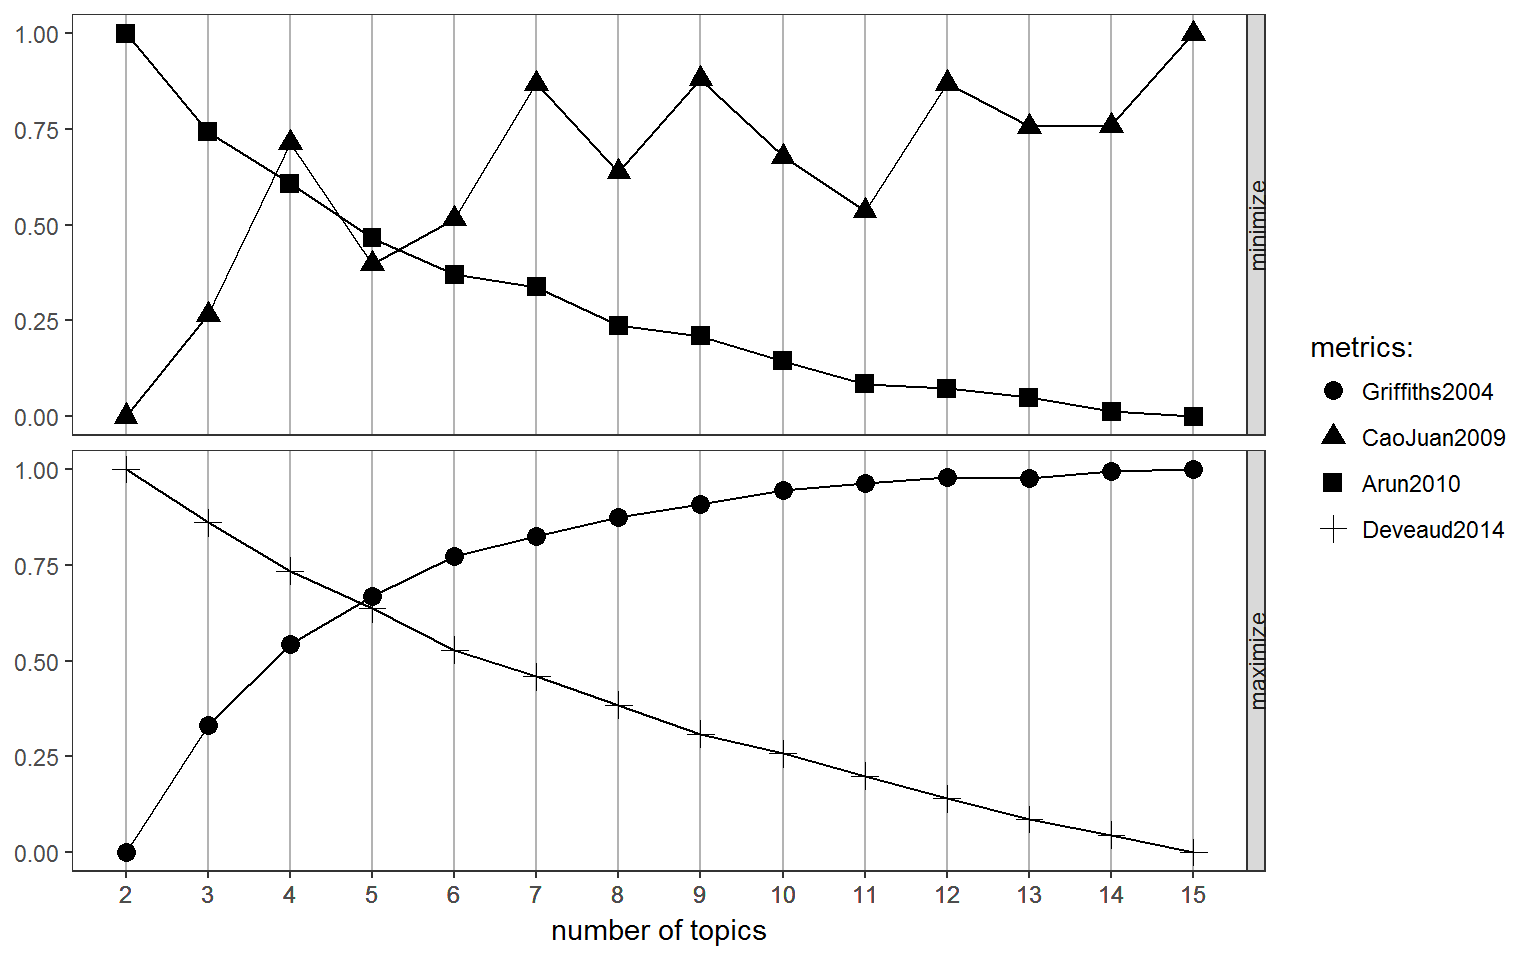
\includegraphics{DSI_Assignment2_Final_Report_files/figure-latex/unnamed-chunk-3-1.pdf}

Overall there is a much tighter grouping of sentences, with less
variation and more conistent lengths, which is useful for techniques
which depend on equal length inputs. The final histogram below shows the
histogram of number of sentences per year/president after filtering,
which still bears the same basic shape as before filtering, but with a
better profile.

\includegraphics{DSI_Assignment2_Final_Report_files/figure-latex/unnamed-chunk-4-1.pdf}

\hypertarget{data-split-and-sampling}{%
\paragraph{Data Split and Sampling}\label{data-split-and-sampling}}

For all group work, we separated our full dataset into a random sampling
of 80\% training and 20\% validation data, which was saved into a common
.RData file. This ensured that there would be consistency across the
data we were working on so that we could use each others work and
compare results more easily.

The graphs above make it clear that our data is also very unbalanced. In
an attempt to correct for this, we applied supersampling with
replacement to the training dataset to ensure an equal number of
sentences per president. Training was attempted using both balanced and
unbalanced training data, but it did not appear to make much difference.
Balancing was conducted on the training dataset only to ensure there are
no duplicates in the validation set that might skew validation error.

\hypertarget{overview-of-the-dataset}{%
\paragraph{\texorpdfstring{\textbf{Overview of the
dataset}}{Overview of the dataset}}\label{overview-of-the-dataset}}

Each president has made a certain number of SONA speeches, depending on
their term in office and whether there was 1 speech that year or 2 in
the year of an election (pre and post election). Since the data is
dependent on their term in the office it is unbalanced. Sentence counts
per president after cleaning the data is :

\begin{verbatim}
## [1] "President sentence counts:"
\end{verbatim}

\begin{verbatim}
## 
##   deKlerk   Mandela     Mbeki Motlanthe Ramaphosa      Zuma 
##       103      1879      2803       346       240      2697
\end{verbatim}

\begin{verbatim}
## [1] "Baseline_accuracies"
\end{verbatim}

\begin{verbatim}
## 
##   deKlerk   Mandela     Mbeki Motlanthe Ramaphosa      Zuma 
##  1.276648 23.289539 34.742191  4.288547  2.974715 33.428359
\end{verbatim}

Let's understand the number of words used by each President and how this
varies across each SONA speech.

\hypertarget{average-number-of-words-used-per-president}{%
\paragraph{\texorpdfstring{\textbf{Average number of words used per
President}}{Average number of words used per President}}\label{average-number-of-words-used-per-president}}

We need to create a metric called ``avg\_words'' which is simply the
total number of words across all SONA speeches made by a particular
president, divided by the total number of SONA speeches that president
made.

\hypertarget{insights}{%
\subsection{\texorpdfstring{\textbf{Insights:}}{Insights:}}\label{insights}}

On average, Mbeki used the most words in his SONA speeches, followed by
Motlanthe and de Klerk used the least. Mandela and Zuma are ranked in
the middle of their peers. The current president (Ramaphosa) used fewer
words than all of his post 1994 peers.

\hypertarget{number-of-words-used-per-sona}{%
\paragraph{\texorpdfstring{\textbf{Number of words used per
SONA}}{Number of words used per SONA}}\label{number-of-words-used-per-sona}}

\hypertarget{insights-1}{%
\subsection{\texorpdfstring{\textbf{Insights:}}{Insights:}}\label{insights-1}}

Of the 3 presidents that have made more than 1 SONA speech, Mbeki used
more words on average than both Mandela and Zuma and the variance in the
number of words used per SONA speech is also higher for Mbeki. In 2004,
which was an election year, the average number of words Mbeki used was
lower in both his pre- and post-election speeches. Towards the end of
his term, his average number of words also dropped off. The data
suggests that perhaps Mbeki's average number of words is correlated with
his confidence in being re-elected President.

\hypertarget{common-words-used-across-all-sona-speeches}{%
\paragraph{\texorpdfstring{\textbf{Common words used across all SONA
speeches}}{Common words used across all SONA speeches}}\label{common-words-used-across-all-sona-speeches}}

\hypertarget{insights-2}{%
\subsection{\texorpdfstring{\textbf{Insights:}}{Insights:}}\label{insights-2}}

\ldots{}.

\hypertarget{common-bigrams-used-across-all-sona-speeches}{%
\paragraph{\texorpdfstring{\textbf{Common bigrams used across all SONA
speeches}}{Common bigrams used across all SONA speeches}}\label{common-bigrams-used-across-all-sona-speeches}}

\hypertarget{insights-3}{%
\subsection{\texorpdfstring{\textbf{Insights:}}{Insights:}}\label{insights-3}}

\ldots{}.

\hypertarget{lexical-diversity-per-president}{%
\paragraph{\texorpdfstring{\textbf{Lexical Diversity per
President}}{Lexical Diversity per President}}\label{lexical-diversity-per-president}}

Lexical diversity refers to the number of unique words used in each
SONA.

\hypertarget{insights-4}{%
\subsection{\texorpdfstring{\textbf{Insights:}}{Insights:}}\label{insights-4}}

The number of unique words per SONA ranges from about 700 with de Klerk
in 1994 to over 2500 with Mandela in his post election speech of 1999.
Mbeki's post election speech of 2004 and Zuma's post election speech of
2014 also got close to the 2500 mark.

It's interesting that whilst the trend in the number of unique words
used was most often upwards with Mandela, Mbeki and Zuma both show a
mostly upward trend in the lead up to the election year, followed by a
mostly downward trend after nearing the 2500 unique words mark in their
post election speech.

If we exclude the post election speeches, the number of unique words
used by Mbeki during his term from 2000 to 2008 averages just under 2000
whereas the number of unique words used by Zuma during his term from
2009 to 2017 averages just over 1500.

\hypertarget{lexical-density-per-president}{%
\paragraph{\texorpdfstring{\textbf{Lexical Density per
President}}{Lexical Density per President}}\label{lexical-density-per-president}}

Lexical density refers to the number of unique words used in each SONA
divided by the total number of words and a high value is an indicator of
word repitition.

\hypertarget{insights-5}{%
\subsection{\texorpdfstring{\textbf{Insights:}}{Insights:}}\label{insights-5}}

De Klerk repeated over 30\% of his words in his 1994 pre election SONA
speech. On average, Mandela repeated about 25\% of words in each of his
SONA speeches and this reduced to about 20\% in the post election speech
of 1999. Mbeki's repitition rate was about 23\% and this reduced to 20\%
in the post election speech of 2004. Zuma's repitition rate is over 30\%
with the exception of his post election speech of 2014 at about 23\%.

\hypertarget{results}{%
\section{\texorpdfstring{\textbf{Results}}{Results}}\label{results}}

\hypertarget{sentiment-analysis}{%
\paragraph{\texorpdfstring{\textbf{Sentiment
Analysis}}{Sentiment Analysis}}\label{sentiment-analysis}}

\hypertarget{analysis-of-sentiment-using-single-words}{%
\subparagraph{\texorpdfstring{\textbf{Analysis of Sentiment using Single
Words}}{Analysis of Sentiment using Single Words}}\label{analysis-of-sentiment-using-single-words}}

\hypertarget{sentiment-analysis-using-bing-lexicon}{%
\subparagraph{\texorpdfstring{\textbf{Sentiment Analysis using ``bing''
lexicon}}{Sentiment Analysis using ``bing'' lexicon}}\label{sentiment-analysis-using-bing-lexicon}}

The ``bing'' lexicon encodes words as either ``positive'' or
``negative''. However, not all words used in the SONA speeches are in
the lexicon so we need to adjust for this.

\hypertarget{sentiment-per-president}{%
\subparagraph{\texorpdfstring{\textbf{Sentiment per
President}}{Sentiment per President}}\label{sentiment-per-president}}

Let's understand how many ``positive'' and ``negative'' words are used
by each president across all their SONA speeches and create a metric
called ``sentiment'' which is simply the total number of positive words
minus the total number of negative words. We then adjust for the total
number of words used from the lexicon in the ``sentiment\_score''
metric.

\textbf{Insights:}

Of the 3 presidents that have made more than 1 SONA speech, Zuma has the
highest sentiment score, followed by Mbeki and then Mandela. Zuma's
sentiment score is nearly double Mandela's. It's interesting that the
current President, Ramaphosa, has the second highest sentiment score,
not far behind Zuma and only slightly ahead of Mbeki.

\hypertarget{what-are-the-10-positive-words-most-frequently-used-by-each-president}{%
\subparagraph{\texorpdfstring{\textbf{What are the 10 positive words
most frequently used by each
president?}}{What are the 10 positive words most frequently used by each president?}}\label{what-are-the-10-positive-words-most-frequently-used-by-each-president}}

\hypertarget{insights-6}{%
\subsection{\texorpdfstring{\textbf{Insights:}}{Insights:}}\label{insights-6}}

De Klerk's most used words were ``freedom'', ``peaceful'' and
``support'' and at least 2 of these 3 come up in all the president's
most used words. Mandela's most used words also include ``progress'',
``improve'', ``reconciliation'' and ``commitment'' which are all words
indicating repair and a move towards something better. Mbeki uses many
of the same words but also introduces ``empowerment'' which is a word
carried through by Zuma and Ramaphosa and ``success'' which is carried
through by Zuma. These words suggest progress in the move towards repair
or something better, first spoken about by Mandela. Ramaphosa also
introduces the words ``confidence'', ``effectively'', ``enhance'' and
``efficient'', which are words commonly seen in a business context and
have not shown up in any other SA president's top 10 most frequently
used words in a SONA since 1994.

\hypertarget{which-of-the-positive-words-most-frequently-used-are-common-across-presidents}{%
\subparagraph{\texorpdfstring{\textbf{Which of the positive words most
frequently used are common across
presidents?}}{Which of the positive words most frequently used are common across presidents?}}\label{which-of-the-positive-words-most-frequently-used-are-common-across-presidents}}

\#\#\textbf{Insights:}

Common positive words across post 1994 presidents include: ``freedom'',
``regard'', ``support'', ``improve'' and ``progress''. Words introduced
by Mandela and unique to his speeches are: ``restructuring'',
``reconciliation'', ``committment'', ``contribution'' and ``succeed''.
Mbeki introduces the words ``empowerment'', ``comprehensive'',
``integrated'' and ``improving'' into the top words used and this is
unique to his speeches. Zuma uses the words ``success'', ``reform'' and
``pleased'' frequently and other presidents do not. Ramaphosa introduces
the words ``significant'', ``productive'', ``confidence'' and
``effectively'' which have not yet been seen in the any other SA
president's top 10 most frequently used words in a SONA since 1994.

\hypertarget{what-are-the-10-negative-words-most-used-by-each-president}{%
\subparagraph{\texorpdfstring{\textbf{What are the 10 negative words
most used by each
president?}}{What are the 10 negative words most used by each president?}}\label{what-are-the-10-negative-words-most-used-by-each-president}}

\#\#\textbf{Insights:}

Common negative words pre 1994 include:
``concerns''/``concern''/``concerned'', ``unconstitutional'',
``illusion'', ``hopeless'', ``disagree'', ``deprive'', ``conflict'', and
``boycott''.

Common negative words post 1994 include: ``corruption'',
``crime''/``criminal'', ``poverty''/``poor'', ``inequality'',
``issue''/``issues'' and ``crisis''.

A negative word introduced by and unique to Mandela's top 10 is
``struggle''. Mbeki is the only president with the word ``racism'' in
his top 10 negative words. Motlanthe has ``conflict'' in his top 10
which no other president does. Zuma has ``rail'' which likely refers to
the railway system and does have negative connotations for South Africa.
Both Zuma and Ramaphosa use the word ``difficult'' a lot. Ramaphosa
introduces the word ``expropriation'' into the top 10 for the first time
amongst his peers.

\hypertarget{how-many-of-the-negative-words-most-used-were-used-by-each-president}{%
\subparagraph{\texorpdfstring{\textbf{How many of the negative words
most used were used by each
president?}}{How many of the negative words most used were used by each president?}}\label{how-many-of-the-negative-words-most-used-were-used-by-each-president}}

\#\#\textbf{Insights:}

The interpretation is much the same as before. Note the clear separation
between the top 10 negative words used pre and post 1994 elections,
indicative of the pre and post apartheid regimes.

\hypertarget{what-proportion-of-words-used-are-positive-vs-negative}{%
\subparagraph{\texorpdfstring{\textbf{What proportion of words used are
positive vs
negative?}}{What proportion of words used are positive vs negative?}}\label{what-proportion-of-words-used-are-positive-vs-negative}}

\#\#\textbf{Insights:}

The 2 vertical black lines are drawn at 60\% amd 70\% positivity rates.
In the majority of years, SONA speeches fall within this range of
positivity however a there are a few more negative speeches in earlier
years and a few more positive speeches in later years.

\hypertarget{change-in-sentiment-over-time}{%
\subparagraph{\texorpdfstring{\textbf{Change in Sentiment over
time}}{Change in Sentiment over time}}\label{change-in-sentiment-over-time}}

\#\#\textbf{Insights:}

The trend appears to be more positive and less negative over time but
how can we be sure?

We will test whether negative sentiment is increasing or decreasing,
then we will test whether positive sentment is increasing or decreasing
. We will use a Binomial model because the frequencies are between 0 and
1. Finally, we will test whether average sentiment is increasing or
decreasing using a linear model.

\hypertarget{is-negative-sentiment-increasing-over-time}{%
\subparagraph{\texorpdfstring{\textbf{Is negative sentiment increasing
over
time?}}{Is negative sentiment increasing over time?}}\label{is-negative-sentiment-increasing-over-time}}

\#\#\textbf{Insights:}

The slope is negative but the beta of the year variable is not
significant so we cannot conclude that negative sentiment is decreasing
over time.

\hypertarget{is-postive-sentiment-increasing-over-time}{%
\subparagraph{\texorpdfstring{\textbf{Is postive sentiment increasing
over
time?}}{Is postive sentiment increasing over time?}}\label{is-postive-sentiment-increasing-over-time}}

\#\#\textbf{Insights:}

The slope is positive but the beta of the year variable is not
significant so we cannot conclude that positive sentiment is increasing
over time.

\hypertarget{is-average-sentiment-increasing-over-time}{%
\subparagraph{\texorpdfstring{\textbf{Is average sentiment increasing
over
time?}}{Is average sentiment increasing over time?}}\label{is-average-sentiment-increasing-over-time}}

\#\#\textbf{Insights:}

The slope is positive and the beta of the year variable is significant
at 1\% so we can conclude that average sentiment is increasing over
time.

But we need to be cautious with this interpretation because what could
actually be going on here is that the ``bing''" lexicon has more than
double the number of negative words than positive words so this could be
influencing the results and SONA speeches may in fact be more positive
than they appear to be.

\hypertarget{distribution-of-bing-sentiment-per-president}{%
\subparagraph{\texorpdfstring{\textbf{Distribution of ``bing'' Sentiment
per
President}}{Distribution of ``bing'' Sentiment per President}}\label{distribution-of-bing-sentiment-per-president}}

\#\#\textbf{Insights:}

Apart from the last 2 presidents, Ramaphosa and Zuma, the presidents are
in time order. We can see that other than Motlanthe, the trend is an
increasing average sentiment over time but at a decreasing rate. The
interquartile range of Mbeki is smaller than Zuma's which is smaller
than Mandela's.

\hypertarget{change-in-bing-sentiment-over-time}{%
\subparagraph{\texorpdfstring{\textbf{Change in ``bing'' Sentiment over
time}}{Change in ``bing'' Sentiment over time}}\label{change-in-bing-sentiment-over-time}}

\#\#\textbf{Insights:}

Average sentiment is the proportion of positive words out of all the
words in the ``bing'' lexicon. Mandela shows a very erratic average
sentiment, ranging from 0 to over 25. Mbeki and Zuma's average sentiment
mostly ranges between 25 and 50, with the exception of a few such as
2000, 2008, 2012, 2017.

\hypertarget{sentiment-analysis-using-afinn-lexicon-scale-from--5-negative-to-5-positive}{%
\subparagraph{\texorpdfstring{\textbf{Sentiment Analysis using ``afinn''
lexicon (scale from -5 negative to +5
positive)}}{Sentiment Analysis using ``afinn'' lexicon (scale from -5 negative to +5 positive)}}\label{sentiment-analysis-using-afinn-lexicon-scale-from--5-negative-to-5-positive}}

\#\#\textbf{Insights:}

The most number of words are scored positive 2, followed by positive 1.
This becomes even more pronounced when scores are multiplied by counts
to get weighted scores.

Let's check the distribution of all ``afinn'' words:

Words with a score of -2 dominate the lexicon, followed by words with a
score of 2. We found a relatively high number of words with a score of 2
in this analysis but it is unlikely to only be a result of its
prevalence in the lexicon and we can conclude that it is probably an
accurate assessment of the sentiment that prevails in the text.

\hypertarget{distribution-of-afinn-sentiment-per-president}{%
\subparagraph{\texorpdfstring{\textbf{Distribution of ``afinn''
Sentiment per
President}}{Distribution of ``afinn'' Sentiment per President}}\label{distribution-of-afinn-sentiment-per-president}}

\#\#\textbf{Insights:}

The interpretation is much the same as with the ``bing'' lexicon in that
the trend is an increasing average sentiment over time however Zuma's
median sentiment is lower than the general trend.

\hypertarget{change-in-afinn-sentiment-over-time}{%
\subparagraph{\texorpdfstring{\textbf{Change in ``afinn'' Sentiment over
time}}{Change in ``afinn'' Sentiment over time}}\label{change-in-afinn-sentiment-over-time}}

\#\#\textbf{Insights:}

Mandela and Zuma show a wave-like pattern of sentiment. Mbeki shows an
increasing and then decreasing pattern.

\hypertarget{sentiment-analysis-using-nrc-lexicon-infers-emotion-with-certain-words}{%
\subparagraph{\texorpdfstring{\textbf{Sentiment Analysis using ``nrc''
lexicon (infers emotion with certain
words)}}{Sentiment Analysis using ``nrc'' lexicon (infers emotion with certain words)}}\label{sentiment-analysis-using-nrc-lexicon-infers-emotion-with-certain-words}}

Let's check the distribution of all ``nrc'' words:

\#\#\textbf{Insights:}

Words can be assigned more than 1 sentiment but we do not expect as many
words to come up under ``anticipation'', ``joy'' or ``surprise'' given
the relatively lower counts in the lexicon. So ``anticipation'' has a
surprisingly high relative count across all presidents.

Given that ``positive'' sentiment is the most frequent classification in
the ``nrc'' lexicon, it is not surprising that it comes out as the most
frequently assigned classification across all presidents. The
distributions across the various sentiments are very similar for all
presidents so this lexicon does not provide any insights about specific
presidents.

\hypertarget{sentiment-analysis-using-nrc-lexicon}{%
\subparagraph{\texorpdfstring{\textbf{Sentiment Analysis using ``nrc''
lexicon}}{Sentiment Analysis using ``nrc'' lexicon}}\label{sentiment-analysis-using-nrc-lexicon}}

\#\#\textbf{Insights:}

The negative most used words which are also associated with the
``anger'', ``disgust'', fear" and ``sadness'' emotions are:
``violence'', ``struggle'' and ``poverty''.

The positive most used words which are also associated with the
``anticipation'', ``joy'' and surprise" emotions are: ``youth'',
``public'' and ``progress''.

The most usedwords that evoke the ``trust'' emotion are: ``system'',
``president'', ``parliament'' and ``nation''.

\hypertarget{topic-modelling}{%
\subsection{\texorpdfstring{\textbf{Topic
Modelling}}{Topic Modelling}}\label{topic-modelling}}

\hypertarget{neural-nets}{%
\subsection{\texorpdfstring{\textbf{Neural Nets
}}{Neural Nets }}\label{neural-nets}}

\hypertarget{neural-net-with-bag-of-words-data}{%
\subsubsection{\texorpdfstring{\textbf{Neural Net with Bag of Words
Data}}{Neural Net with Bag of Words Data}}\label{neural-net-with-bag-of-words-data}}

The count of each word that have been used in each sentence is what we
are going to be feeding in. We need to unnest the sentence data, count
each word in each sentence and spread the sentence word counts so that
we have sentence id's in each row and we have each word as column id's.
This is the simplest neural net model that we can try, so that was our
first model.

This model has L2 regularization to avoid overfitting but even so it
didn't help very much. The accuracy is 0.55886. The optimizer\_rmsprop
has learning rate 0.003. This was choosen after trying lr=c(0.001,
0.002, 0.003) To make readability easier the model with best learning
rate is used.

As we can see from the plot model overfits after the second iteration,
since the loss function start increasing in value, so to avoid that
let's use a smaller model with less neurons and add a dropout.

\#\#\#\#\textbf{Cohen's Kappa}

Kappa value tells you how much better your classifier is performing over
the performance of a classifier that simply guesses at random according
to the frequency of each class.

``Cohen?s kappa is always less than or equal to 1. Values of 0 or less,
indicate that the classifier is useless. There is no standardized way to
interpret its values. Landis and Koch (1977) provide a way to
characterize values. According to their scheme a value \textless{} 0 is
indicating no agreement , 0???0.20 as slight, 0.21???0.40 as fair,
0.41???0.60 as moderate, 0.61???0.80 as substantial, and 0.81???1 as
almost perfect agreement.'' {[}Reference: Landis, J.R.; Koch, G.G.
(1977). ???The measurement of observer agreement for categorical
data???. Biometrics 33 (1): 159???174{]}

The accuracy is slightly better than bigger model with no-dropouts
(0.581\%) Just for the word-count model seems good enough. But this
model does not consider how important each word is to its corpus. So we
should consider a better model to try.

After the fourth iteration validation loss starts increasing which is a
sign of overfitting.

\hypertarget{neural-net-with-tf-idf-data}{%
\subsubsection{\texorpdfstring{\textbf{Neural Net with tf-idf
Data}}{Neural Net with tf-idf Data}}\label{neural-net-with-tf-idf-data}}

TFIDF is a statisic that shows how important a word is to it's corpus.
So if we are feeding NN with TFIDF we are logically expecting the
results to be slightly better than the word-cout NN model.

\#\#\#\#\textbf{Cohen's Kappa}

The accuracy is 0.6158 and the model starts overfitting after fourth
epoch. So this is slightly better than the bag of words word-count model
as we expected.

\#\#\#\textbf{Neural Net with Sentiment Analysis Data}

\#\#\#\#\textbf{Cohen's Kappa}

Sentiment analysis also reaches it's smallest validation loss value on
the fifth iteration. But the train accuracy and test accuracy is
changing very slightly at each iteration. This model does not seem to be
doing well on eighter the training set or the test set. The test
accuracy is 0.4361834 and the training accuracy is 0.4353395. If we look
at the NRC sentiment lexicon it is visible that all presidents share
same sentiment distribution pattern, so this is why it is not
overfitting. Because our set aside test set is actually no different
than the training set.

\#\#\#\textbf{Neural Nets with Topic Modelling Data (Gamma Values)}

Topic modelling only predicted for president 1(Mbeki) and president
2(Zuma).

\#\#\#\#\textbf{Cohen's Kappa}

The train and the test set are not very distinct from each other just
like sentiment analysis. If we look at the mixture of the topics by each
president in topic modelling chunk we can see that all the topics for
each president are kind of uniformed and hard to seperate each
president's topic from one another.

\#\#\#\textbf{CNN with Transfer Learning \n(Pre-trained Embeddings)}

We will be using GloVe embeddings. GloVe stands for ``Global Vectors for
Word Representation'' and is an unsupervised learning algorithm for
obtaining vector representations for words as it is stated in their
website. Training is performed on aggregated global word-word
co-occurrence statistics from a corpus, and the resulting
representations showcase interesting linear substructures of the word
vector space. {[}Reference:Jeffrey Pennington, Richard Socher, and
Christopher D. Manning. 2014. GloVe: Global Vectors for Word
Representation:\url{https://nlp.stanford.edu/pubs/glove.pdf} {]}
Specifically, we will use the 100-dimensional GloVe embeddings of 400k
words computed on a 2014 dump of English Wikipedia.

This note is taken from the reference given above and as they state the
accuracy they achieved on python is twice as good.

``IMPORTANT NOTE:This example does yet work correctly. The code executes
fine and appears to mimic the Python code upon which it is based however
it achieves only half the training accuracy that the Python code does so
there is clearly a subtle difference. We need to investigate this
further before formally adding to the list of examples''

{[}reference for implementation on Python:
\url{https://blog.keras.io/using-pre-trained-word-embeddings-in-a-keras-model.html}{]}
{[}reference for implementation on R:
\url{https://keras.rstudio.com/articles/examples/pretrained_word_embeddings.html}{]}
{[}reference for implementation on R:
\url{https://github.com/rstudio/keras/blob/master/vignettes/examples/pretrained_word_embeddings.R}{]}

Also for the pre-trained embeddings to work well it needs to be trained
with similar type of data that you are trying to classify, and the fact
that the GloVe embeddings are trained on Wikipedia data one can expect
that it would not neccesarily help predict the presidents better for our
sentences.

Majority of the sentences of Mbeki is predicted as Mandela(379/569).
Majority of the sentences of Zuma is predicted as Mandela (244/534) and
the secon majority is predicted as himself (195/534). Majority of the
sentences of Mandela is predicted as Mandela(263/381). Majority of the
sentences of Mothlane(38/66) is predicted as Mandela. Majority of
sentences of Ramaphosa is predicted as Mandela(19/47) or Zuma(15/47).
Mojority of the sentences of deKlerk is predicted as Mandela(14/17).

\#\#\#\#\textbf{Cohen's Kappa}

\hypertarget{neural-net-nn-to-predict-the-president-from-a-sentence}{%
\subsection{\texorpdfstring{\textbf{Neural Net (nn) to predict the
President from a
Sentence}}{Neural Net (nn) to predict the President from a Sentence}}\label{neural-net-nn-to-predict-the-president-from-a-sentence}}

\hypertarget{evaluate-out-of-sample-performance}{%
\paragraph{\texorpdfstring{\textbf{Evaluate Out of Sample
Performance}}{Evaluate Out of Sample Performance}}\label{evaluate-out-of-sample-performance}}

test\_acc

\hypertarget{convolutional-neural-net-cnn-to-predict-the-president-from-a-sentence}{%
\subsection{\texorpdfstring{\textbf{Convolutional Neural Net (cnn) to
predict the President from a
Sentence}}{Convolutional Neural Net (cnn) to predict the President from a Sentence}}\label{convolutional-neural-net-cnn-to-predict-the-president-from-a-sentence}}

\hypertarget{evaluate-out-of-sample-performance-1}{%
\subsubsection{\texorpdfstring{\textbf{Evaluate Out of Sample
Performance}}{Evaluate Out of Sample Performance}}\label{evaluate-out-of-sample-performance-1}}

\hypertarget{recurrent-neural-net-rnn-to-predict-president-from-sentence}{%
\paragraph{\texorpdfstring{\textbf{Recurrent Neural Net (rnn) to predict
President from
Sentence}}{Recurrent Neural Net (rnn) to predict President from Sentence}}\label{recurrent-neural-net-rnn-to-predict-president-from-sentence}}

\hypertarget{evaluate-out-of-sample-performance-2}{%
\paragraph{\texorpdfstring{\textbf{Evaluate Out of Sample
Performance}}{Evaluate Out of Sample Performance}}\label{evaluate-out-of-sample-performance-2}}

here we can combine all the train and test accuracies in a table, as a
conclusion.

\hypertarget{analysis-of-results-and-conclusion}{%
\subsection{\texorpdfstring{\textbf{Analysis of Results and
Conclusion}}{Analysis of Results and Conclusion}}\label{analysis-of-results-and-conclusion}}

Also done the critisism after each chunk.

\hypertarget{references}{%
\subsection{\texorpdfstring{\textbf{References}}{References}}\label{references}}

\url{https://www.kaggle.com/rtatman/tutorial-sentiment-analysis-in-r}

\url{https://www.datacamp.com/community/tutorials/sentiment-analysis-R}

\url{https://nlp.stanford.edu/pubs/glove.pdf}

\url{https://blog.keras.io/using-pre-trained-word-embeddings-in-a-keras-model.html}

\url{https://keras.rstudio.com/articles/examples/pretrained_word_embeddings.html}

\url{https://github.com/rstudio/keras/blob/master/vignettes/examples/pretrained_word_embeddings.R}

Landis, J.R.; Koch, G.G. (1977). ???The measurement of observer
agreement for categorical data???. Biometrics 33 (1): 159???174


\end{document}
